%%%
%
% $Autor: Siddhanth Sharma $
% $Date: 2024-10-31 11:15:45Z $
% $File: file.tex $
% $Version: 1 $
%
% Project: 
%
%%%

\chapter{Streamlit}
\label{ch:streamlit}

\section{Introduction}

\textbf{Streamlit} is the deployment library used to transform the CPI forecasting workflow into an interactive analytical application. In this project, the package is not responsible for training the models; instead, it acts as the presentation and interaction layer above already-trained ARIMA, ETS, and SARIMA models \cite{streamlit-doc}. This separation is important because it keeps model estimation in the offline pipeline and reserves the app for reproducible visualization and interpretation.

\section{Description}

The complete \textbf{Streamlit} implementation is located in \FILELOC{Code/app.py}. The application loads the cleaned CPI data, reads serialized model objects from \FILELOC{Code/saved\_models/}, computes forecasts for the 24-month test horizon, and displays both plots and error metrics. Users can select a single forecasting model or switch to a comparison mode in which all three models are shown simultaneously.

Several \textbf{Streamlit} features are used directly in the app:

\begin{itemize}
    \item \texttt{st.sidebar.selectbox()} for model and confidence-interval selection,
    \item \texttt{st.metric()} for RMSE, MAE, and MAPE presentation,
    \item \texttt{st.plotly\_chart()} for interactive forecast visualizations,
    \item \texttt{st.expander()} for explanatory text,
    \item \texttt{st.warning()} and \texttt{st.error()} for user-facing failure messages,
    \item \texttt{@st.cache\_data} for efficient data loading.
\end{itemize}

This package is therefore relevant not only for deployment convenience, but also for communicating model behavior to non-technical users.

Table~\ref{tab:streamlit-ui-elements} summarizes the main user-interface elements implemented in the dashboard.

\begin{table}[htbp]
    \centering
    \caption{Main Streamlit interface elements in the CPI dashboard.}
    \label{tab:streamlit-ui-elements}
    {\small
    \renewcommand{\arraystretch}{1.22}
    \setlength{\tabcolsep}{7pt}
    \begin{tabular}{L{4.2cm}L{8.7cm}}
        \hline
        UI element & Purpose \\
        \hline
        Sidebar model selector & Chooses the forecasting view shown to the user \\
        Confidence-interval selector & Adjusts the displayed uncertainty level for forecast intervals \\
        Metric display area & Presents RMSE, MAE, and MAPE in compact form \\
        Plotly chart area & Visualizes actual and forecast CPI values interactively \\
        Expanders and warning messages & Support interpretation and communicate runtime issues \\
        \hline
    \end{tabular}
    }
\end{table}

\section{Installation}

\textbf{Streamlit} is included in the project dependency file:

\begin{Python}[caption={Installing project dependencies including Streamlit}, label={lst:install_streamlit_project}]
pip install -r Code/requirements.txt
\end{Python}

If installed separately, the command is:

\begin{Python}[caption={Installing Streamlit directly}, label={lst:install_streamlit_direct}]
pip install streamlit
\end{Python}

The installation can be checked as follows:

\begin{Python}[caption={Verifying the Streamlit installation}, label={lst:verify_streamlit}]
import streamlit as st
print(st.__version__)
\end{Python}

\section{Example -- Description}

A concrete project example is the model-comparison view in \FILELOC{Code/app.py}. In this mode, \textbf{Streamlit} loads all saved models, recomputes RMSE, MAE, and MAPE on the common holdout period, highlights the best metric values in a table, and renders an interactive Plotly chart with actual and predicted CPI values. This turns the static evaluation from the modeling pipeline into an exploratory interface that can be used during demonstration and interpretation.

\section{Example -- Manual}

The dashboard can be started with the following practical sequence:

\begin{enumerate}
    \item Install all Python dependencies from \FILELOC{Code/requirements.txt}.
    \item Run \FILELOC{Code/src/modeling\_pipeline.py} first so that the model files exist in \FILELOC{Code/saved\_models/}.
    \item Start the app with \SHELL{streamlit run Code/app.py} from the project root.
    \item Open the local \textbf{Streamlit} URL shown in the terminal.
    \item Select a forecasting model or choose \texttt{Compare All Models}.
    \item Inspect forecast curves, confidence intervals, and evaluation metrics.
\end{enumerate}

\section{Example -- Code}

\begin{Python}[caption={Typical Streamlit controls used in the CPI dashboard}, label={lst:streamlit_project_code}]
st.sidebar.header("Configuration")
model_choice = st.sidebar.selectbox(
    "Select Model",
    ["ARIMA (1,1,1)", "ETS (A,A,A)", "SARIMA (1,1,1)x(1,1,1,12)", "Compare All Models"]
)

ci_level = st.sidebar.selectbox("Confidence Interval Level", [80, 90, 95, 96, 97, 98, 99], index=2)
\end{Python}

This excerpt illustrates how Streamlit exposes forecasting settings as user-selectable controls without requiring code modification by the end user.

\section{Example -- Files}

The main files and artifacts connected to Streamlit are:

\begin{itemize}
    \item \FILELOC{Code/app.py} -- complete Streamlit application.
    \item \FILELOC{Code/saved\_models/*.joblib} -- pretrained models loaded at runtime.
    \item \FILELOC{Code/data/61111-0002\_en.csv} -- CPI data source used in the app.
\end{itemize}

\section{Package Role in the CPI Pipeline}

The following figure should be read as a package-level deployment view rather than as a replacement for the KDD diagram in Chapter~\ref{ch:kdd-methodology}. Whereas the KDD chapter explains the overall analytical methodology from data selection to evaluation, this figure isolates the role of \textbf{Streamlit} after the modeling stage has already produced reusable artifacts. In practice, the package belongs closest to the report's deployment and presentation layers: it loads the CPI data together with the saved models, exposes user controls for model and confidence-interval selection, triggers forecast and metric generation for the chosen view, and renders the dashboard that makes the forecasting results accessible for interpretation. The left-to-right structure of the figure is therefore meant to reflect the actual interaction sequence experienced by the user in the application.

\begin{figure}[htbp]
\centering
\resizebox{0.95\linewidth}{!}{
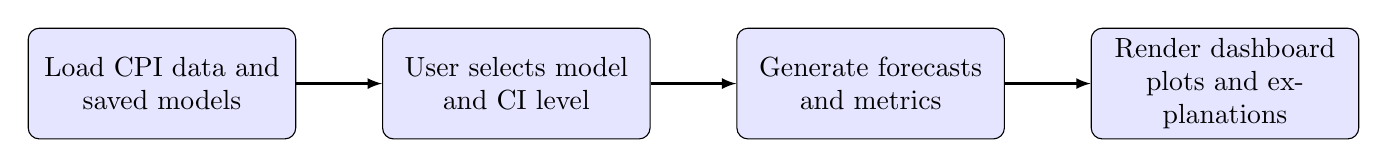
\begin{tikzpicture}[
    block/.style={rectangle, draw, fill=blue!10, text width=9em, text centered, rounded corners, minimum height=4em},
    line/.style={draw, -latex, thick}
]
    \node [block] (load) at (0,0) {Load CPI data and\\saved models};
    \node [block] (select) at (4.5,0) {User selects model\\and CI level};
    \node [block] (forecast) at (9,0) {Generate forecasts\\and metrics};
    \node [block] (display) at (13.5,0) {Render dashboard\\plots and explanations};

    \draw [line] (load) -- (select);
    \draw [line] (select) -- (forecast);
    \draw [line] (forecast) -- (display);
\end{tikzpicture}
}
\caption{Package-level view of \textbf{Streamlit} within the CPI pipeline. The figure complements the KDD methodology by showing the downstream deployment and presentation layer in which previously trained artifacts are loaded, configured by the user, used to generate forecasts and metrics, and displayed as an interactive dashboard.}
\label{fig:streamlit_workflow}
\end{figure}

\section{Further Reading}

\begin{itemize}
    \item Streamlit documentation: \URL{https://docs.streamlit.io/}
    \item Streamlit API reference: \URL{https://docs.streamlit.io/library/api-reference}
\end{itemize}
